\documentclass{article}
%% FROM THE PROVIDED math_symbols.tex
\usepackage{amsthm}
\usepackage{amssymb}
\usepackage{amsmath}
\usepackage{mathtools}
\usepackage{xifthen}
\usepackage{xparse}
\usepackage{dsfont}


% Left-right bracket
\newcommand{\lr}[1]{\left (#1\right)}

% Left-right square bracket
\newcommand{\lrs}[1]{\left [#1 \right]}

% Left-right curly bracket
\newcommand{\lrc}[1]{\left \{#1\right\}}

% Left-right absolute value
\newcommand{\lra}[1]{\left |#1\right|}

% Left-right upper value
\newcommand{\lru}[1]{\left \lceil#1\right\rceil}

% Scalar product
\newcommand{\vp}[2]{\left \langle #1 , #2 \right \rangle}

% The real numbers
\newcommand{\R}{\mathbb R}

% The natural numbers
\newcommand{\N}{\mathbb N}

% Expectation symbol with an optional argument
\NewDocumentCommand{\E}{o}{\mathbb E\IfValueT{#1}{\lrs{#1}}}

% Indicator function with an optional argument
\NewDocumentCommand{\1}{o}{\mathds 1{\IfValueT{#1}{\lr{#1}}}}

% Probability function
\let\P\undefined
\NewDocumentCommand{\P}{o}{\mathbb P{\IfValueT{#1}{\lr{#1}}}}

% A hypothesis space
\newcommand{\HH}{\mathcal H}

% A sample space
\newcommand{\XX}{\mathcal{X}}

% A label space
\newcommand{\YY}{\mathcal{Y}}

% A nicer emptyset symbol
\let\emptyset\varnothing

% Sign operator
\DeclareMathOperator{\sign}{sign}
\newcommand{\sgn}[1]{\sign\lr{#1}}

% KL operator
\DeclareMathOperator{\KL}{KL}

% kl operator
\DeclareMathOperator{\kl}{kl}

% The entropy
\let\H\relax
\DeclareMathOperator{\H}{H}

% Majority vote
\DeclareMathOperator{\MV}{MV}

% Variance
\DeclareMathOperator{\V}{Var}
\NewDocumentCommand{\Var}{o}{\V\IfValueT{#1}{\lrs{#1}}}

% VC
\DeclareMathOperator{\VC}{VC}

% VC-dimension
\newcommand{\dVC}{d_{\VC}}

% FAT ...
\DeclareMathOperator{\FAT}{FAT}
\newcommand{\dfat}{d_{\FAT}}
\newcommand{\lfat}{\ell_{\FAT}}
\newcommand{\Lfat}{L_{\FAT}}
\newcommand{\hatLfat}{\hat L_{\FAT}}

% Distance
\DeclareMathOperator{\dist}{dist}

% change all asterisks to \cdots in math mode. use \textasciiasterisk for
% asterisks in math mode.
\DeclareMathSymbol{*}{\mathbin}{symbols}{"01}

% easy integrals over -infinty .. infinity
\newcommand{\infint}{\int\limits_{-\infty}^{\infty}}


%% MY PACKAGES
\usepackage[utf8]{inputenc}
\usepackage[plainpages=false]{hyperref}
\usepackage{cleveref}
\usepackage{graphicx}
\usepackage{minted}    % code snippets
\usemintedstyle{trac}
\setminted{fontsize=\scriptsize, highlightcolor=gray, linenos, frame=lines, framesep=10pt}
% \usepackage{tikz}
% \usetikzlibrary{automata, positioning}
\usepackage[]{xcolor}
\definecolor{gray}{RGB}{235, 230, 222}
\definecolor{myRed}{RGB}{173, 20, 0}
\definecolor{myGreen}{RGB}{45, 150, 0}
\newcommand{\gray}[1]{{\setlength{\fboxsep}{0pt}\colorbox{gray}{#1}}}
\everymath{\displaystyle} % force display style for inline math. why though?


%% My COMMANDS
% big, fat, red TODO's.
\newcommand{\TODO}[1]{\textcolor{red}{TODO: #1}}

\newcommand\numberthis{\addtocounter{equation}{1}\tag{\theequation}} % equation numbering for align*

%% math related commands/operators.

% neat section and subsection separators (but have to insert manually).
\newcommand{\sectend}{\smallskip\noindent\makebox[\textwidth]{\rule{\textwidth}{0.4pt}}}
\newcommand{\Sectend}{\medskip\noindent\makebox[\textwidth]{\rule{1.1\textwidth}{1pt}}}

% easy monospace text for inline code. also,
% no need to escape underscores as with \texttt.
\newcommand{\ms}[1]{\mintinline[fontsize=\normalsize]{text}{#1}}

\DeclareMathOperator*{\argmin}{argmin}

\newcommand{\mbf}[1]{\mathbf{#1}}
\usepackage{geometry}


\author{\texttt{sortraev} (Anders Holst)}

\title{AADS 2022/23 -- exam
  \ifdef{\notes}{
    \ifdef{\presentations}{
      % both notes and presentations.
      notes\\ and presentations
    }
    { % just notes.
      notes
    }
  }{
    % just presentations.
    presentations
  }
}

\setcounter{tocdepth}{2}
\begin{document}

\maketitle
\newpage
\tableofcontents
\newpage

\ifdef{\notes}{
\section{Notes}
\subsection{Max flow}

\paragraph{Disposition}
\begin{itemize}
\item intro.
\item Ford-Fulkerson.
\item Edmonds-Karp.
\item proof: Edmonds-Karp in $O(|V| * |E|^2)$.
\end{itemize}

\paragraph{Notes}

\begin{enumerate}
  \item hello.
  \item motivation: routing, bipartite matching, image segmentation.
  \item (define problem?)
  \item state assumptions ($|f|$, res. net., augmentation, flow cancellation,
    etc.).\\

  \item Ford-Fulkerson.
  \item Edmonds-Karp.
  \item draw example (below).
  \item proof: Edmonds-Karp runtime.
\end{enumerate}

\begin{figure}[H]
  \centering
  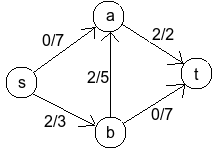
\includegraphics[width=0.6\textwidth]{figures/max_flow_example.png}
  \caption{Max flow example.}
  \label{fig:max_flow_example}
\end{figure}
 % X2
\newpage

\subsection{Linear programming and optimization}

\paragraph{Disposition}
\begin{itemize}
  \item intro.
  \item standard and slack form.
  \item small example of transforming LP problem to standard and slack forms.
  \item SIMPLEX algorithm and duality.
  \item prove weak duality.
\end{itemize}

\paragraph{Notes}

\begin{enumerate}
  \item hello.

  \item linear programming and constraint optimization.\\

  \item \emph{draw example} and explain constituents.

  \item standard form \emph{(give formula)}.

  \item slack form.\\

  \item \emph{example: one iteration of SIMPLEX.}

  \item dual LP program \emph{(give formula)}.

  \item proof of weak duality AND COROLLARY.
\end{enumerate}

\begin{alignat*}{3}
  \text{minimize } \quad& -2x_1 && +3 x_2  \quad&\\
  \text{s.t.     } \quad& x_1   && + x_2   \quad&=\quad 7\\
                        & x_1   && -2x_2   \quad&\leq\quad 4\\
                        & x_1   &&         \quad&\geq \quad0
\end{alignat*}

\newpage

\subsection{Randomized algorithms}


\paragraph{Disposition}

\begin{itemize}
  \item hello and intro.
  \item motivation.

  \item Las Vegas vs Monte Carlo.
  \item regular quicksort and its worst case complexity.

  \item LV example: RandQS.
  \item proof: \#comparisons made by RandQS.

  \item MC examle: RAND\_MIN\_CUT.
  \item proof: probabilistic error-bound for RAND\_MIN\_CUT.
\end{itemize}



\paragraph{Notes}

\begin{enumerate}
  \item hello.

  \item motivation for randomization.

  \item Las Vegas and Monte Carlo.

  \item regular quicksort: pivoting and complexities.

  \item LV example: RandQS -- strategy and complexity.

  \item proof: \#comparisons made by RandQS.

  \item MC example: RAND\_MIN\_CUT -- strategy.
  \item proof:probabilistic error-bound for RAND\_MIN\_CUT.
\end{enumerate}


\newpage
\subsubsection{Pseudocode}

\paragraph{RandQS}

\begin{minted}{text}
RandQS(S):
    if |S| <= 1:
        return S
    pivot = pick at uniform random an item in S;
            remove it from S and use it as pivot.
    S_l = {x in S : x <= pivot}
    S_r = {x in S : x >  pivot}
    return RandQS(S_l) ++ [pivot] ++ RandQS(S_r)
\end{minted}

\paragraph{Randomized min-cut}

\begin{minted}{text}
RAND_MIN_CUT(V, E):
    V' = {MAKE-SET(v) : v in V}

    C  = empty set
    E' = random permutation of E
    n = |V'|
    for (u, v) in E':
        p_u = find(u)
        p_v = find(v)
        if p_u != p_v:
            if n > 2 then:
                UNION(p_u, p_v)
                n -= 1
            else:
                C += (u, v)

    return C
\end{minted}
 % mangler
\newpage
\subsection{Hashing}

\begin{enumerate}
  \item hello.

  \item motivation: variable- to fixed-length keys; unordered sets. Is often
    used to speed up algorithms which require sets or associative arrays; for
    example used to improve space complexity of vEB-trees from $O(|U|)$ to $O(n
    \lg \lg |U|)$ (at the cost of expected $O(\lg \lg |U|)$ time updates).

  \item a random hashing function \textcolor{red}{$h : U \mapsto [m]$} is a
    function mapping values from a larger set to a (possibly, but not
    necessarily) smaller set $[m]$. For pratical purposes, we typically require
    that $[m]$ is bounded and that the values are fixed size/length. \emph{In
    addition, note that if $[m]$ is larger than $U$, then the task of hashing is
    trivial, as will likely be the benefits.}

  \item if we are using random hashing, then for each $x \in U$ the hash
    \textcolor{red}{$h(x) \in [m]$} is a random variable.

  \item when picking a random hash function $h$, we are often interested in the
    space needed to represent $h$; the time is takes to compute $h(x)$ (given $x
    \in U$); and the properties of the underlying RV.

  \item today, we shall primarily discuss the latter (the randomness in
    hashing).

  \item ideally, we would want a hashing function that is \emph{truly random},
    ie. $h(x) \neq h(y)$ for any distinct keys $x$ and $y$ in $U$. Due to space
    necessities, however, this is impractical, since designing such a hashing
    function that holds for all inputs requires one to encode an output for
    every possible input, which means a total of $m^{|U|}$ hashing functions in
    one!

    This would eliminate one of the primary motivations for hashing, which is to
    represent an element from a huge range in a smaller range.

  \item introduce \textbf{c-approximate universality}. A random hash function $h
    : U \mapsto [m]$ is $c$-approximately universal if for all distinct keys $x$
    and $y$ in $U$, the probability that they hash similarly is $\leq c/m$,
    where $m = |\,[m]\,|$:
    \begin{textred}
      \begin{align}
        \forall x \neq y \in U\ :\ \prh{h(x) = h(y)} \leq c/m.
      \end{align}
    \end{textred}

  \item similarly, we define \textbf{c-approximate \emph{strong} universality}
    as: a random hash function $h : U \mapsto [m]$ is $c$-approximately strongly
    universal if each key $x \in U$ is hashed $c$-approximately uniformly into
    $[m]$:
    \begin{textred}
      \begin{align}
        \forall x \in U,\ q \in [m]\ :\ \prh{h(x) = q}\quad \leq\quad c/m.
      \end{align}
    \end{textred}

    and if any two distinct keys hash independently, ie.:

    \begin{textred}
      \begin{align}
        \forall x \neq y \in U,\text{ and } q, r \in [m]\ :\ \prh{h(x) = q\
        \land\ h(y) = r} \quad\leq\quad (c/m)^2.
      \end{align}
    \end{textred}

  \item in either case we require $c$ to be $O(1)$ (and ideally small), and
    when $c = 1$, we simply say the given function is ``universal'' or
    ``strongly universal''.

  \item some examples of hashing functions are: 

    \begin{enumerate}

      \begin{textgray}
      \item the \textbf{universal multiply-mod-prime}: choose a prime number $p \geq
        |U|$, and pick uniformly random integers $a \in [p]_+$ and $b \in [p]$.
        Then multiply-mod-prime is defined by:

          \begin{align}
            h_{a, b} = ((ax + b) \mod p) \mod m.
          \end{align}
      \end{textgray}


      \item The \textbf{2-approximately universal multiply-shift}: 

        When hashing from $w$ to $l$ bits: pick at uniformly random an odd
        $w$-bit integer $a$ and define $h_a : [2^w] \mapsto [2^\ell]$ as such:

        \begin{textred}
          \begin{align}
            h_a(x) = \left\lfloor\, \frac{ax \mod 2^w} {2^{w - \ell}} \,\right\rfloor.
          \end{align}
        \end{textred}

        \begin{textgray}
        which compensates for its lack in universality compared to
        multiply-mod-prime with its speed in practical implementation.
        \end{textgray}

      \item The \textbf{strongly universal multiply-shift}:

        When hashing from $w$ to $l$ bits: choose a $\bar w \geq w + \ell - 1$,
        and pick at uniformly random $a, b \in [2^{\bar w}]$. Then define $h_{a,
        b}$ as such:

        \begin{textred}
        \begin{align}
          h_{a, b}    &: [2^w] \mapsto [2^\ell]\\[6pt]
          h_{a, b}(x) &= \left\lfloor \frac{(ax + b) \mod 2^{\bar w}} {2^{\bar
          w - \ell}}\right\rfloor
        \end{align}
        \end{textred}

    \end{enumerate}
      \item so far, so good. Now, I want to present an example application of
        random hashing, in which strong universality provides a big benefit.

      \item the example is \emph{coordinated sampling}. Given a universe $U$ of
        samples, we imagine $k$ independent, but possibly overlapping subsets
        $A_1, \dots, A_k \subseteq U$. These $k$ subsets may each be of enormous
        size and hence for each subset, we take an even smaller sample $S_{h,
        t}(A_i)$, where $h$ is some strongly universal hashing function from $U$
        to $[m]$ and $t \in [m]$. Then the sample $S(A) = S_{h, t}(A)$ is given
        by:
        \begin{textred}
          \begin{align}
            S(A_i) = S_{h, t}(A_i) = \{a \in A_i \ :\  h(a) < t\}.
          \end{align}
        \end{textred}

        In other words, an element $a$ is sampled from $A_i$ if its hash wrt.
        $h$ is below the chosen threshold.

      \item since $h$ is chosen to be strongly universal (ie. we have pairwise
        independence between samples), the chance of any element in $A_i$
        hashing to any given value in $[m]$ is $1/m$, and because we sample an
        element if it hashes below $t$, the probability of any $a \in A_i$ being
        sampled is $t / m$.

        \emph{This part only requires universality, but strong universality
        implies universality, so we are good.}

      \item if the same $h$ and $t$ are used in all of the $k$ subsets of $U$,
        then two samples can be used to examine likeness between the subsets
        they are sampled from:

        \begin{textred}
          \begin{align}
            \forall 1 \leq i, j \leq k\ : a \in A_i \land a \in A_j \implies a
            \in S_{h, t}(A_i) \iff S_{h, t}(A_j).
          \end{align}
        \end{textred}

        in other words, if an element is in two subsets, then it is sampled from
        one subset \textbf{iff} it is also sampled from the other, so long as
        the same $h$ and $t$ are used to sample from either subset. 

 
      \item another useful fact is that $S(A_i)$ can be used to estimate the
        size of $A_i$. Let's see how:

        If the sampling probability is $t/m$, then the expected size of $S(A)$
        is $t/m * |A|$:

        \begin{textred}
        \begin{alignat*}{4}
                                             & |S(A)| \ &&\simeq \ \frac{t}{m} * |A|\\
          \Leftrightarrow \quad \frac{m}{t}\ & |S(A)| \ &&\simeq \ |A|.
        \end{alignat*}
        \end{textred}

        In fact, because $h$ is (strongly) universal, we have an unbiased
        estimate of the size of $S(A)$:

        \begin{textred}
        \begin{align}
          \mu = \E{|S(A)|} = \frac{t}{m} * |A|.
        \end{align}
        \end{textred}

      \item if $h$ is also strongly universal, then we can use Chebyshev's
        inequality to put a probabilistic bound the quality of this estimate.

        Recall Chebyshev's inequality. If $X$ is iid with $X \in [0, 1]$ and
        unbiased estimator $\E{X} = \mu$, and standard deviation $\sigma$, then
        for $q > 0$:

        \begin{textred}
          \begin{align}
            \text{Pr}\big[|X - \mu | \geq q \sigma\big] \quad \leq \quad \frac{1}{q^2}.
          \end{align}
        \end{textred}

        and $\text{Var}(X) \leq \mu$.

      \item in our case, if we let $X_a = [h(a) < t]$ be an indicator variable
        for whether the element $a \in A$ is sampled under $h$ and $t$, then the
        sum $X = \sum_{a \in A} X_a = |S(A)|$ is an RV with $\mu \geq
        \text{Var}(X)$ and hence $\sqrt{\mu} \geq \sqrt{\text{Var}(X)} =
        \sigma$.

      \item let $a = |A|$ for brevity. To summarize, we have $X = S(A)$, $\mu =
        at/m$, and $\sqrt{\mu} = \sqrt{at/m} \geq \sigma$, and can thus apply Chebyshev's:

        \begin{textred}
          \begin{align}
            \text{Pr}\left[\Big\vert|S(A)| - \frac{t}{m} a
            \Big\vert \geq q * \sqrt{\frac{t}{m}a}\right] \quad \leq \quad
            \frac{1}{q^2}.
          \end{align}
        \end{textred}

\end{enumerate}
 % fin
\newpage
\subsection{Van Emde Boas trees}

\paragraph{Disposition}
\begin{itemize}
\item motivation and intuition.

\item small example (two insertions and a successor query).

\item $T(u) \leq T(\sqrt[\uparrow]{u}) + O(1)\ \in\ O(\lg \lg u)$.

\item illustrate how vEB operations follow this recurrence (examples for
  insert and successor).

\end{itemize}



\paragraph{Notes}

\begin{enumerate}

  \item hello.

  \item motivation for and intuition behind vEB trees.

  \item time and space complexity.\\

  \item vEB recurrence: $T(u) \leq T(\sqrt[\uparrow]{u}) + O(1)$.

  \item example for $U = 8$ (see \cref{fig:veb_example}).

  \item show $T(u) \leq T(\sqrt[\uparrow]{u}) + O(1) \in O(\lg \lg u)$.

  \item show how this recurrence describes vEB operations (insert and successor).

\end{enumerate}

\begin{figure}[H]
  \centering
  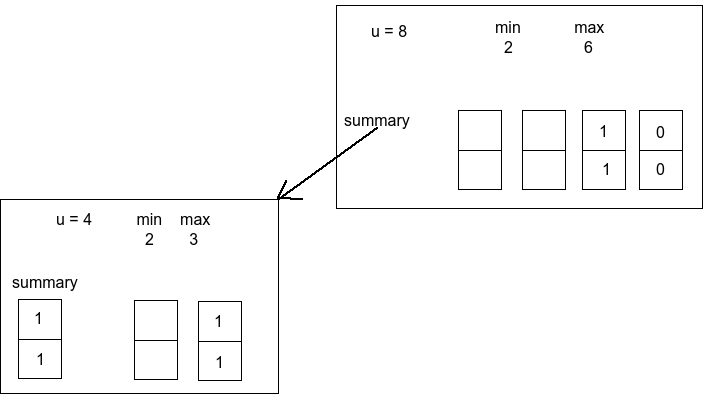
\includegraphics[width=0.7\textwidth]{figures/veb_example.png}
  \caption{Example -- vEB tree containing keys \{2, 5, 6\}.}
  \label{fig:veb_example}
\end{figure}
 % kunne godt bruge en tur mere

\newpage
\subsection{NP-completeness}

\begin{enumerate} \item what is a ``hard'' problem? answer: we think of ``hard''
      as something which cannot be solved in polynomial time.

  \item today we will be discussing the NP-complete class of problems. These are
    decision problems which: can be verified in polynomial time (NP) and which
    are at least as hard as all other problems in NP (NP-hard).

    \begin{textred}
      \begin{align}
        \text{NP-complete}
        \begin{cases}
          \text{NP}\\
          \text{NP-hard}
        \end{cases}
      \end{align}
    \end{textred}

  \item I am going to show NP-completeness of the k-vertex cover problem, and,
    if there is time, the decision variant of the traveling salesperson problem.

  \item first, I want to define three terms: languages, verifiability, and
    reducibility.

  \item in an effort to formalize the concept of a ``problem'', we use the
    framework of \emph{languages}, that is, strings of characters from some
    given alphabet. For our purposes, the language will be strings of zeroes and
    ones:

      \begin{textred}
      \begin{align}
        \Sigma^\ast = \{0, 1\}^\ast.
      \end{align}
      \end{textred}

  \item next is verifiability. For a lot of problems, we are able to verify a
    possible solution as fast as or faster than computing a new solution from
    scratch.

    Verifiability requires a ``certificate'' string, here called $y$, describing
    a solution to the given input string, which can be checked using a
    verification algorithm, here called $A$.

    If for a given language we know how to verify a string in time polynomial
    in the size of that string, then we say that the language belongs to NP:
      \begin{textred}
      \begin{align}
        L = \{x \in \Sigma^\ast\ :\ \exists y  \in \Sigma^\ast \ . \ |y| =
        O(|x|^c) \ .\  A(x, y) = 1\}.
      \end{align}
      \end{textred}
    For some languages, however, verifying a solution might take superpolynomial
    time, sometimes because it involves computing the solution string from
    scratch (example: TSP).

  \item the last is reducibility. Often when we analyze the complexity of a
    problem, or language, we ``reduce'' the language to be an instance of
    another language for which we know the complexity.

  \item we say that a language $L'$ is reducible to another language $L$ if an
    instance of $L'$ can be transformed into an instance of $L$. Ideally, we
    want this transformation to be possible in polynomial time, and we say that
    a language $L'$ is polynomial-time reducible to $L$ if there exists a
    polynomial-time computable function $f : \Sigma^\ast$ satisfying:

    \begin{textred}
    \begin{align}
       x \in L' \iff f(x) \in L.
    \end{align}
    \end{textred}

    if so, then we say that \textcolor{red}{$L' \leq_P L$}.

  \item \TODO{something missing here!!!!!!!!!!!!!!}

  \item example: k-vertex cover. If you are not familiar with the vertex cover
    problem \emph{and/or its decision variant}, please let me know now.

  \item I will show k-vertex cover is in NP-hard by reducing CLIQUE, which we know
    to be NP-complete, to k-vertex cover.

    What I propose is: $G$ has a clique of size $k$ \textbf{iff} its complement
    graph $\bbar G$ has a vertex cover of size $|V| - k$. In other words:
    CLIQUE($G$, $k$) has a solution \textbf{iff} VERTEX-COVER($\bbar G$, $|V| -
    k$) has a solution.

  \item assume CLIQUE($G$, $k$) has a solution $V'$ of size $k$.

  \item consider an edge \red{$e = (u, v) \in \bbar E$}. Then $e$ cannot be in
    $E$ and we have:

    \begin{textred}
    \begin{align}
      e \not \in E \implies u \not \in V' \text{ or } v \not \in V',
    \end{align}
    \end{textred}

    since $u$ and $v$ cannot both be in the clique if they do not share an edge.
    If any of them are not in the clique, then they are in the complement set:
    
    \begin{textred}
    \begin{align}
      u \in V \setminus V' \text{ or } v \in V \setminus V'
    \end{align}
    \end{textred}

    since at least one of $u$ or $v$ is in the complement set, we say that the
    edge $(u, v)$ is \emph{covered} by the complement set $V \setminus V'$.

  \item Since this holds for any $e \in \bbar E$, the complement graph $\bbar G$
    is a cover of size:

      \begin{textred}
      \begin{align}
        |V \setminus V'| = |V| - |V'| = |V| - k.
      \end{align}
      \end{textred}

  \item We will now show the backwards direction of the bi-implication. Assume
    that the complement graph $\bbar G$ has a vertex cover $V'$ of size $|V| -
    k$.

    For all $u, v \in V$, if $(u, v) \in \bbar E$ then at least one of its
    endpoints must be in $V'$:

    \begin{textred}
    \begin{align}
        \forall u, v \in V\ :\ (u, v) \in \bbar E \implies u \in V' \text{ or } v \in V'
    \end{align}
    \end{textred}

    since at least one of $u$ or $v$ must cover the edge.

    The contrapositive of this expression is:

    \begin{textred}
    \begin{align}
        \forall u, v \in V\ :\ u \not \in V' \text{ and } v \not \in V' \implies
        (u, v) \not \in \bbar E \iff (u, v) \in E,
    \end{align}
    \end{textred}

    and hence we have \red{$(u, v) \in E$}.

  \item constructing the complement graph takes \red{$O(|V|^2)$} time, hence the
    reduction takes polynomial time.\\[4pt]


  \item next up, if there is still time, is the traveling salesperson problem or
    TSP. Regular TSP is NP-hard but not NP, and hence we consider instead the
    decision variant of the problem, which is NP-complete, as we shall also see.

  \item if you are not familiar with TSP or its decision variant, please shout
    now! In any case, we define the language TSP to be:

    \begin{textred}
      \begin{align}
        \text{TSP} = \{(G, c, k)\ :\ &\ G \text{ complete},\\
                                   \ &\ c\, :\ V \times V \mapsto \mathbb R,\\
                                   \ &\ k \in \mathbb N \cup \{0\},\\
                                   \ &\ G \text{ has a tour of cost} \leq k\}.
    \end{align}
    \end{textred}

  \item let's show that TSP is NP-complete. First, we show that TSP is in NP by
    describing a possible certificate as such: the certificate is a sequence of
    $|V|$ vertices. The verification checks that the graph is complete, and if
    it is, then any sequence of distinct vertices form a simple cycle.
    Verification then checks that each vertex in $G$ is represented exactly once
    in the certificate, and that the weight of the cycle is $\leq k$.

  \item checking graph completeness takes \textcolor{red}{$O(|V|^2)$} time, and
    checking the cycle and computing its weight takes \textcolor{red}{$O(|V|)$}
    time.

  \item we will show NP-hardness by reducing HAM-CYCLE to TSP. The
    transformation of the input problem goes as such: let $G = (V, E)$. Then
    \textcolor{red}{HAM-CYCLE($G$) has a solution \textbf{iff} TSP($G'$, $c'$,
    0) has a solution}, where $G'$ is the completion of $G$ and
    \textcolor{red}{$c'(i, j) = [(v_i, v_j) \not \in E] * \infty$}. As such the
    weight of an edge in $E'$ is 0 if it is also an edge in $E$; else it is
    infinite. We could also assign a weight of 1 to edges not in $E$.

  \item assume HAM-CYCLE($G$) has a solution. Let one such hamiltonian cycle in
    $G$ be called $h$. Since $h$ contains only edges in $E$, it has weight 0.
    Since $E'$ is a superset of $E$, $h$ is also a hamiltonian cycle in $E'$.
    Hence there is a cycle of weight $\leq 0$ in $G'$, satisfying TSP($G'$,
    $c'$, 0).

    Assume now that TSP($G'$, $c'$, 0) has a solution. Let one such cycle of
    weight $\leq 0$ be called $h$. Since $h$ has weight $\leq 0$ and all edges
    are non-negative, all edges in $h$ must be 0. Then, since only edges in $E$
    have weight 0, all edges in $h$ must be in $E$ as well. Hence $G$ has a
    hamiltonian cycle.

  \item constructing the complete graph $G'$ takes \textcolor{red}{$O(|V|^2)$}
    time. Hence the reduction is polynomial time.

\end{enumerate}
 % X2
\newpage

\subsection{Exact exponential algorithms and FPT}


\paragraph{Disposition}
\begin{itemize}
\item motivation (EEA vs PC vs approximation)
\item O-star notation
\item exact exponential algorithm example: traveling salesperson problem
\item parameterized complexity example: vertex-cover problem.
\end{itemize}


\paragraph{Notes}

\begin{enumerate}
  \item hello.
  \item EEA and FPT.
  \item fast, universal, exact.\\
  \item first: EEA.
  \item EEA for NP problems.
  \item EEA for NP-hard problems.
  \item big-O-star notation (??).
  \item TSP; naive time and space complexity.
  \item Held-Karp: bottom-up DP.
  \item $\OPT(S, v_i)$ -- $S$ and $v_i$.
  \item TIME and SPACE of $\OPT(S, v_i)$.\\
  \item FPT -- idea and motivation.
  \item k-VC; non-FPT polynomial solution.
  \item FPT+kernelization and its complexity.
\end{enumerate}

\paragraph{Pseudocode}
\label{code:tsp}

\begin{minted}[escapeinside=@@, linenos=true, frame=lines]{text}
TSP({c@$_1$@, .., c@$_n$@}, d):
  for i = 2 .. n:
    OPT[{c@$_i$@}, c@$_i$@] = d(c@$_1$@, c@$_i$@)
  for j = 2 .. n - 1:
    for every subset S of {c@$_2$@, .., c@$_n$@} with |S| = j:
      for c@$_i$@ in S:
        OPT[S, c_i] = min{OPT[S', c@$_k$@] + d(c@$_k$@, c@$_i$@)
                          : c@$_k$@ in S' = S @\textbackslash@ {c@$_i$@}}
  return min{OPT[{c@$_2$@, .., c@$_n$@}, c@$_i$@] + d(c@$_i$@, c@$_1$@)
             : c@$_i$@ in {c@$_2$@, .., c@$_n$@}}
\end{minted}


\newpage

\subsection{Approximation algorithms}

\paragraph{Disposition}

\begin{itemize}
  \item hello and intro.
  \item motivation.
  \item approximation ratio.\\
  \item FPTAS
  \item FPTAS example: APPROX-SUBSET-SUM.
  \item if time: 2-approximate vertex-cover.
\end{itemize}

\paragraph{Notes}

\begin{enumerate}
  \item hello.
  \item motivation: speed over exactness.
  \item approximation ratio.
  \item approximation schemes: PTAS and FPTAS.\\

  \item SUBSET-SUM and APPROX-SUBSET-SUM.
  \item example: APPROX-SUBSET-SUM([3, 50, 2, 40], 89, 0.1).\\

  \item proof: APPROX-SUBSET-SUM is FPTAS.
    \begin{enumerate}
      \item feasible solution.
      \item $(1 + \eps)$ approximation ratio.
      \item poly runtime.
    \end{enumerate}
\end{enumerate}

\newpage
\subsubsection{Pseudocode: SUBSET-SUM and FPTAS-SUBSET-SUM}
\label{sec:fptas_subset_sum_pseudocode}

\begin{minted}[escapeinside=@@, linenos=true, frame=lines]{text}
SUBSET-SUM(S, t):
  L@$_0$@ = [0]
  n = |S|
  for k = 1 .. n:
    L@$_k$@ = MERGE(L@$_{k-1}$@, [x in L@$_{k-1}$@ : x + s@$_k$@])
    L@$_k$@ = [x in L@$_k$@ : x <= t]
  return last(L@$_n$@)
\end{minted}



\begin{minted}[escapeinside=@@, linenos=true, frame=lines]{text}
FPTAS-SUBSET-SUM(S, t, @$\eps$@):
  L'@$_0$@ = [0]
  n = |S|
  for k = 1 .. n:
    L'@$_k$@ = MERGE(L'@$_{k-1}$@, [x in L'@$_{k-1}$@ : x + s@$_k$@])
    L'@$_k$@ = TRIM(L'@$_k$@, @$\eps$@ / (2 * n))
    L'@$_k$@ = [x in L'@$_k$@ : x <= t]
  return last(L'@$_n$@)
\end{minted}

\begin{minted}[escapeinside=@@, linenos=true, frame=lines]{text}
TRIM(S, @$\delta$@):
  m = |S|
  if m == 0:
      return S
  L = [s@$_1$@]
  for i = 2 .. m:
    if s@$_i$@ > last(L) * @$\delta$@:
      L = APPEND(L, s@$_i$@)
  return L
\end{minted}

 % X2
\newpage

\subsection{Polygon triangulation}

\paragraph{Disposition}

\begin{itemize}
  \item hello, intro, and motivation.
  \item triangulation and monotonicity.
  \item algorithms and their complexities.
  \item proof: MAKE\_MONOTONE.
  \item proof: size of monotone decomposition.
\end{itemize}

\paragraph{Notes}

\begin{enumerate}
  \item hello.
  \item motivation: computer graphics, computational geometry.

  \item describe triangulation and (y-)monotonicity.

  \item $n := |V|$.

  \item TRIANGULATE\_MONOTONE\_POLYGON in $O(n)$ time.
  \item MAKE\_MONOTONE in $O(n \lg n)$ time.

  \item show MAKE\_MONOTONE partitions $P$ into monotone subpolygons \\(for
    HANDLE\_SPLIT\_VERTEX only) with only legal diagonals.
  \item show size of monotone decomposition is $O(n)$.
\end{enumerate}

\begin{figure}[H]
  \centering
  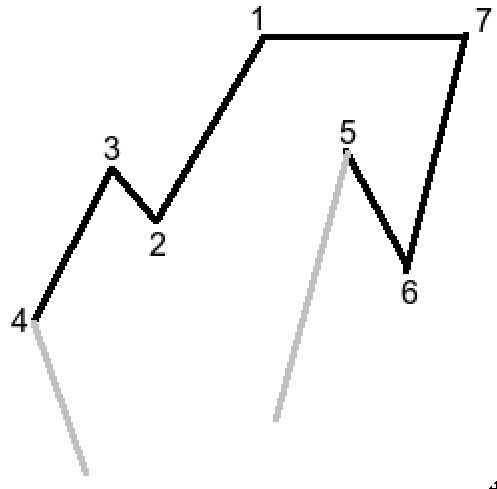
\includegraphics[width=0.5\textwidth]{figures/monotonization_example.png}
  \caption{Polygon monotonization example.}
  \label{fig:monotonization_example}
\end{figure}

}{}

\ifdef{\presentations}
{
\section{Presentations}
\subsection{Max flow}

\paragraph{Disposition}
\begin{itemize}
\item intro.
\item Ford-Fulkerson.
\item Edmonds-Karp.
\item proof: Edmonds-Karp in $O(|V| * |E|^2)$.
\end{itemize}

\paragraph{Notes}

\begin{enumerate}
  \item hello.
  \item motivation: routing, bipartite matching, image segmentation.
  \item (define problem?)
  \item state assumptions ($|f|$, res. net., augmentation, flow cancellation,
    etc.).\\

  \item Ford-Fulkerson.
  \item Edmonds-Karp.
  \item draw example (below).
  \item proof: Edmonds-Karp runtime.
\end{enumerate}

\begin{figure}[H]
  \centering
  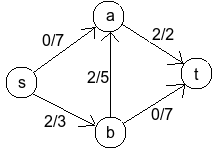
\includegraphics[width=0.6\textwidth]{figures/max_flow_example.png}
  \caption{Max flow example.}
  \label{fig:max_flow_example}
\end{figure}

\newpage

\subsection{Linear programming and optimization}

\paragraph{Disposition}
\begin{itemize}
  \item intro.
  \item standard and slack form.
  \item small example of transforming LP problem to standard and slack forms.
  \item SIMPLEX algorithm and duality.
  \item prove weak duality.
\end{itemize}

\paragraph{Notes}

\begin{enumerate}
  \item hello.

  \item linear programming and constraint optimization.\\

  \item \emph{draw example} and explain constituents.

  \item standard form \emph{(give formula)}.

  \item slack form.\\

  \item \emph{example: one iteration of SIMPLEX.}

  \item dual LP program \emph{(give formula)}.

  \item proof of weak duality AND COROLLARY.
\end{enumerate}

\begin{alignat*}{3}
  \text{minimize } \quad& -2x_1 && +3 x_2  \quad&\\
  \text{s.t.     } \quad& x_1   && + x_2   \quad&=\quad 7\\
                        & x_1   && -2x_2   \quad&\leq\quad 4\\
                        & x_1   &&         \quad&\geq \quad0
\end{alignat*}

\newpage

\subsection{Randomized algorithms}


\paragraph{Disposition}

\begin{itemize}
  \item hello and intro.
  \item motivation.

  \item Las Vegas vs Monte Carlo.
  \item regular quicksort and its worst case complexity.

  \item LV example: RandQS.
  \item proof: \#comparisons made by RandQS.

  \item MC examle: RAND\_MIN\_CUT.
  \item proof: probabilistic error-bound for RAND\_MIN\_CUT.
\end{itemize}



\paragraph{Notes}

\begin{enumerate}
  \item hello.

  \item motivation for randomization.

  \item Las Vegas and Monte Carlo.

  \item regular quicksort: pivoting and complexities.

  \item LV example: RandQS -- strategy and complexity.

  \item proof: \#comparisons made by RandQS.

  \item MC example: RAND\_MIN\_CUT -- strategy.
  \item proof:probabilistic error-bound for RAND\_MIN\_CUT.
\end{enumerate}


\newpage
\subsubsection{Pseudocode}

\paragraph{RandQS}

\begin{minted}{text}
RandQS(S):
    if |S| <= 1:
        return S
    pivot = pick at uniform random an item in S;
            remove it from S and use it as pivot.
    S_l = {x in S : x <= pivot}
    S_r = {x in S : x >  pivot}
    return RandQS(S_l) ++ [pivot] ++ RandQS(S_r)
\end{minted}

\paragraph{Randomized min-cut}

\begin{minted}{text}
RAND_MIN_CUT(V, E):
    V' = {MAKE-SET(v) : v in V}

    C  = empty set
    E' = random permutation of E
    n = |V'|
    for (u, v) in E':
        p_u = find(u)
        p_v = find(v)
        if p_u != p_v:
            if n > 2 then:
                UNION(p_u, p_v)
                n -= 1
            else:
                C += (u, v)

    return C
\end{minted}

\newpage
\subsection{Hashing}

\begin{enumerate}
  \item hello.

  \item motivation: variable- to fixed-length keys; unordered sets. Is often
    used to speed up algorithms which require sets or associative arrays; for
    example used to improve space complexity of vEB-trees from $O(|U|)$ to $O(n
    \lg \lg |U|)$ (at the cost of expected $O(\lg \lg |U|)$ time updates).

  \item a random hashing function \textcolor{red}{$h : U \mapsto [m]$} is a
    function mapping values from a larger set to a (possibly, but not
    necessarily) smaller set $[m]$. For pratical purposes, we typically require
    that $[m]$ is bounded and that the values are fixed size/length. \emph{In
    addition, note that if $[m]$ is larger than $U$, then the task of hashing is
    trivial, as will likely be the benefits.}

  \item if we are using random hashing, then for each $x \in U$ the hash
    \textcolor{red}{$h(x) \in [m]$} is a random variable.

  \item when picking a random hash function $h$, we are often interested in the
    space needed to represent $h$; the time is takes to compute $h(x)$ (given $x
    \in U$); and the properties of the underlying RV.

  \item today, we shall primarily discuss the latter (the randomness in
    hashing).

  \item ideally, we would want a hashing function that is \emph{truly random},
    ie. $h(x) \neq h(y)$ for any distinct keys $x$ and $y$ in $U$. Due to space
    necessities, however, this is impractical, since designing such a hashing
    function that holds for all inputs requires one to encode an output for
    every possible input, which means a total of $m^{|U|}$ hashing functions in
    one!

    This would eliminate one of the primary motivations for hashing, which is to
    represent an element from a huge range in a smaller range.

  \item introduce \textbf{c-approximate universality}. A random hash function $h
    : U \mapsto [m]$ is $c$-approximately universal if for all distinct keys $x$
    and $y$ in $U$, the probability that they hash similarly is $\leq c/m$,
    where $m = |\,[m]\,|$:
    \begin{textred}
      \begin{align}
        \forall x \neq y \in U\ :\ \prh{h(x) = h(y)} \leq c/m.
      \end{align}
    \end{textred}

  \item similarly, we define \textbf{c-approximate \emph{strong} universality}
    as: a random hash function $h : U \mapsto [m]$ is $c$-approximately strongly
    universal if each key $x \in U$ is hashed $c$-approximately uniformly into
    $[m]$:
    \begin{textred}
      \begin{align}
        \forall x \in U,\ q \in [m]\ :\ \prh{h(x) = q}\quad \leq\quad c/m.
      \end{align}
    \end{textred}

    and if any two distinct keys hash independently, ie.:

    \begin{textred}
      \begin{align}
        \forall x \neq y \in U,\text{ and } q, r \in [m]\ :\ \prh{h(x) = q\
        \land\ h(y) = r} \quad\leq\quad (c/m)^2.
      \end{align}
    \end{textred}

  \item in either case we require $c$ to be $O(1)$ (and ideally small), and
    when $c = 1$, we simply say the given function is ``universal'' or
    ``strongly universal''.

  \item some examples of hashing functions are: 

    \begin{enumerate}

      \begin{textgray}
      \item the \textbf{universal multiply-mod-prime}: choose a prime number $p \geq
        |U|$, and pick uniformly random integers $a \in [p]_+$ and $b \in [p]$.
        Then multiply-mod-prime is defined by:

          \begin{align}
            h_{a, b} = ((ax + b) \mod p) \mod m.
          \end{align}
      \end{textgray}


      \item The \textbf{2-approximately universal multiply-shift}: 

        When hashing from $w$ to $l$ bits: pick at uniformly random an odd
        $w$-bit integer $a$ and define $h_a : [2^w] \mapsto [2^\ell]$ as such:

        \begin{textred}
          \begin{align}
            h_a(x) = \left\lfloor\, \frac{ax \mod 2^w} {2^{w - \ell}} \,\right\rfloor.
          \end{align}
        \end{textred}

        \begin{textgray}
        which compensates for its lack in universality compared to
        multiply-mod-prime with its speed in practical implementation.
        \end{textgray}

      \item The \textbf{strongly universal multiply-shift}:

        When hashing from $w$ to $l$ bits: choose a $\bar w \geq w + \ell - 1$,
        and pick at uniformly random $a, b \in [2^{\bar w}]$. Then define $h_{a,
        b}$ as such:

        \begin{textred}
        \begin{align}
          h_{a, b}    &: [2^w] \mapsto [2^\ell]\\[6pt]
          h_{a, b}(x) &= \left\lfloor \frac{(ax + b) \mod 2^{\bar w}} {2^{\bar
          w - \ell}}\right\rfloor
        \end{align}
        \end{textred}

    \end{enumerate}
      \item so far, so good. Now, I want to present an example application of
        random hashing, in which strong universality provides a big benefit.

      \item the example is \emph{coordinated sampling}. Given a universe $U$ of
        samples, we imagine $k$ independent, but possibly overlapping subsets
        $A_1, \dots, A_k \subseteq U$. These $k$ subsets may each be of enormous
        size and hence for each subset, we take an even smaller sample $S_{h,
        t}(A_i)$, where $h$ is some strongly universal hashing function from $U$
        to $[m]$ and $t \in [m]$. Then the sample $S(A) = S_{h, t}(A)$ is given
        by:
        \begin{textred}
          \begin{align}
            S(A_i) = S_{h, t}(A_i) = \{a \in A_i \ :\  h(a) < t\}.
          \end{align}
        \end{textred}

        In other words, an element $a$ is sampled from $A_i$ if its hash wrt.
        $h$ is below the chosen threshold.

      \item since $h$ is chosen to be strongly universal (ie. we have pairwise
        independence between samples), the chance of any element in $A_i$
        hashing to any given value in $[m]$ is $1/m$, and because we sample an
        element if it hashes below $t$, the probability of any $a \in A_i$ being
        sampled is $t / m$.

        \emph{This part only requires universality, but strong universality
        implies universality, so we are good.}

      \item if the same $h$ and $t$ are used in all of the $k$ subsets of $U$,
        then two samples can be used to examine likeness between the subsets
        they are sampled from:

        \begin{textred}
          \begin{align}
            \forall 1 \leq i, j \leq k\ : a \in A_i \land a \in A_j \implies a
            \in S_{h, t}(A_i) \iff S_{h, t}(A_j).
          \end{align}
        \end{textred}

        in other words, if an element is in two subsets, then it is sampled from
        one subset \textbf{iff} it is also sampled from the other, so long as
        the same $h$ and $t$ are used to sample from either subset. 

 
      \item another useful fact is that $S(A_i)$ can be used to estimate the
        size of $A_i$. Let's see how:

        If the sampling probability is $t/m$, then the expected size of $S(A)$
        is $t/m * |A|$:

        \begin{textred}
        \begin{alignat*}{4}
                                             & |S(A)| \ &&\simeq \ \frac{t}{m} * |A|\\
          \Leftrightarrow \quad \frac{m}{t}\ & |S(A)| \ &&\simeq \ |A|.
        \end{alignat*}
        \end{textred}

        In fact, because $h$ is (strongly) universal, we have an unbiased
        estimate of the size of $S(A)$:

        \begin{textred}
        \begin{align}
          \mu = \E{|S(A)|} = \frac{t}{m} * |A|.
        \end{align}
        \end{textred}

      \item if $h$ is also strongly universal, then we can use Chebyshev's
        inequality to put a probabilistic bound the quality of this estimate.

        Recall Chebyshev's inequality. If $X$ is iid with $X \in [0, 1]$ and
        unbiased estimator $\E{X} = \mu$, and standard deviation $\sigma$, then
        for $q > 0$:

        \begin{textred}
          \begin{align}
            \text{Pr}\big[|X - \mu | \geq q \sigma\big] \quad \leq \quad \frac{1}{q^2}.
          \end{align}
        \end{textred}

        and $\text{Var}(X) \leq \mu$.

      \item in our case, if we let $X_a = [h(a) < t]$ be an indicator variable
        for whether the element $a \in A$ is sampled under $h$ and $t$, then the
        sum $X = \sum_{a \in A} X_a = |S(A)|$ is an RV with $\mu \geq
        \text{Var}(X)$ and hence $\sqrt{\mu} \geq \sqrt{\text{Var}(X)} =
        \sigma$.

      \item let $a = |A|$ for brevity. To summarize, we have $X = S(A)$, $\mu =
        at/m$, and $\sqrt{\mu} = \sqrt{at/m} \geq \sigma$, and can thus apply Chebyshev's:

        \begin{textred}
          \begin{align}
            \text{Pr}\left[\Big\vert|S(A)| - \frac{t}{m} a
            \Big\vert \geq q * \sqrt{\frac{t}{m}a}\right] \quad \leq \quad
            \frac{1}{q^2}.
          \end{align}
        \end{textred}

\end{enumerate}

\newpage
\subsection{Van Emde Boas trees}

\paragraph{Disposition}
\begin{itemize}
\item motivation and intuition.

\item small example (two insertions and a successor query).

\item $T(u) \leq T(\sqrt[\uparrow]{u}) + O(1)\ \in\ O(\lg \lg u)$.

\item illustrate how vEB operations follow this recurrence (examples for
  insert and successor).

\end{itemize}



\paragraph{Notes}

\begin{enumerate}

  \item hello.

  \item motivation for and intuition behind vEB trees.

  \item time and space complexity.\\

  \item vEB recurrence: $T(u) \leq T(\sqrt[\uparrow]{u}) + O(1)$.

  \item example for $U = 8$ (see \cref{fig:veb_example}).

  \item show $T(u) \leq T(\sqrt[\uparrow]{u}) + O(1) \in O(\lg \lg u)$.

  \item show how this recurrence describes vEB operations (insert and successor).

\end{enumerate}

\begin{figure}[H]
  \centering
  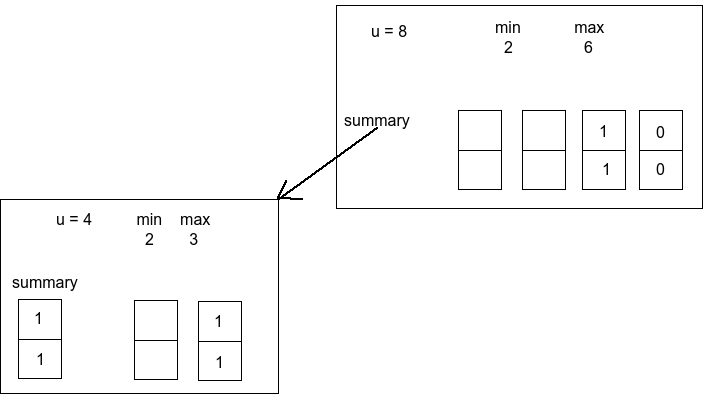
\includegraphics[width=0.7\textwidth]{figures/veb_example.png}
  \caption{Example -- vEB tree containing keys \{2, 5, 6\}.}
  \label{fig:veb_example}
\end{figure}

\newpage
\subsection{NP-completeness}

\begin{enumerate} \item what is a ``hard'' problem? answer: we think of ``hard''
      as something which cannot be solved in polynomial time.

  \item today we will be discussing the NP-complete class of problems. These are
    decision problems which: can be verified in polynomial time (NP) and which
    are at least as hard as all other problems in NP (NP-hard).

    \begin{textred}
      \begin{align}
        \text{NP-complete}
        \begin{cases}
          \text{NP}\\
          \text{NP-hard}
        \end{cases}
      \end{align}
    \end{textred}

  \item I am going to show NP-completeness of the k-vertex cover problem, and,
    if there is time, the decision variant of the traveling salesperson problem.

  \item first, I want to define three terms: languages, verifiability, and
    reducibility.

  \item in an effort to formalize the concept of a ``problem'', we use the
    framework of \emph{languages}, that is, strings of characters from some
    given alphabet. For our purposes, the language will be strings of zeroes and
    ones:

      \begin{textred}
      \begin{align}
        \Sigma^\ast = \{0, 1\}^\ast.
      \end{align}
      \end{textred}

  \item next is verifiability. For a lot of problems, we are able to verify a
    possible solution as fast as or faster than computing a new solution from
    scratch.

    Verifiability requires a ``certificate'' string, here called $y$, describing
    a solution to the given input string, which can be checked using a
    verification algorithm, here called $A$.

    If for a given language we know how to verify a string in time polynomial
    in the size of that string, then we say that the language belongs to NP:
      \begin{textred}
      \begin{align}
        L = \{x \in \Sigma^\ast\ :\ \exists y  \in \Sigma^\ast \ . \ |y| =
        O(|x|^c) \ .\  A(x, y) = 1\}.
      \end{align}
      \end{textred}
    For some languages, however, verifying a solution might take superpolynomial
    time, sometimes because it involves computing the solution string from
    scratch (example: TSP).

  \item the last is reducibility. Often when we analyze the complexity of a
    problem, or language, we ``reduce'' the language to be an instance of
    another language for which we know the complexity.

  \item we say that a language $L'$ is reducible to another language $L$ if an
    instance of $L'$ can be transformed into an instance of $L$. Ideally, we
    want this transformation to be possible in polynomial time, and we say that
    a language $L'$ is polynomial-time reducible to $L$ if there exists a
    polynomial-time computable function $f : \Sigma^\ast$ satisfying:

    \begin{textred}
    \begin{align}
       x \in L' \iff f(x) \in L.
    \end{align}
    \end{textred}

    if so, then we say that \textcolor{red}{$L' \leq_P L$}.

  \item \TODO{something missing here!!!!!!!!!!!!!!}

  \item example: k-vertex cover. If you are not familiar with the vertex cover
    problem \emph{and/or its decision variant}, please let me know now.

  \item I will show k-vertex cover is in NP-hard by reducing CLIQUE, which we know
    to be NP-complete, to k-vertex cover.

    What I propose is: $G$ has a clique of size $k$ \textbf{iff} its complement
    graph $\bbar G$ has a vertex cover of size $|V| - k$. In other words:
    CLIQUE($G$, $k$) has a solution \textbf{iff} VERTEX-COVER($\bbar G$, $|V| -
    k$) has a solution.

  \item assume CLIQUE($G$, $k$) has a solution $V'$ of size $k$.

  \item consider an edge \red{$e = (u, v) \in \bbar E$}. Then $e$ cannot be in
    $E$ and we have:

    \begin{textred}
    \begin{align}
      e \not \in E \implies u \not \in V' \text{ or } v \not \in V',
    \end{align}
    \end{textred}

    since $u$ and $v$ cannot both be in the clique if they do not share an edge.
    If any of them are not in the clique, then they are in the complement set:
    
    \begin{textred}
    \begin{align}
      u \in V \setminus V' \text{ or } v \in V \setminus V'
    \end{align}
    \end{textred}

    since at least one of $u$ or $v$ is in the complement set, we say that the
    edge $(u, v)$ is \emph{covered} by the complement set $V \setminus V'$.

  \item Since this holds for any $e \in \bbar E$, the complement graph $\bbar G$
    is a cover of size:

      \begin{textred}
      \begin{align}
        |V \setminus V'| = |V| - |V'| = |V| - k.
      \end{align}
      \end{textred}

  \item We will now show the backwards direction of the bi-implication. Assume
    that the complement graph $\bbar G$ has a vertex cover $V'$ of size $|V| -
    k$.

    For all $u, v \in V$, if $(u, v) \in \bbar E$ then at least one of its
    endpoints must be in $V'$:

    \begin{textred}
    \begin{align}
        \forall u, v \in V\ :\ (u, v) \in \bbar E \implies u \in V' \text{ or } v \in V'
    \end{align}
    \end{textred}

    since at least one of $u$ or $v$ must cover the edge.

    The contrapositive of this expression is:

    \begin{textred}
    \begin{align}
        \forall u, v \in V\ :\ u \not \in V' \text{ and } v \not \in V' \implies
        (u, v) \not \in \bbar E \iff (u, v) \in E,
    \end{align}
    \end{textred}

    and hence we have \red{$(u, v) \in E$}.

  \item constructing the complement graph takes \red{$O(|V|^2)$} time, hence the
    reduction takes polynomial time.\\[4pt]


  \item next up, if there is still time, is the traveling salesperson problem or
    TSP. Regular TSP is NP-hard but not NP, and hence we consider instead the
    decision variant of the problem, which is NP-complete, as we shall also see.

  \item if you are not familiar with TSP or its decision variant, please shout
    now! In any case, we define the language TSP to be:

    \begin{textred}
      \begin{align}
        \text{TSP} = \{(G, c, k)\ :\ &\ G \text{ complete},\\
                                   \ &\ c\, :\ V \times V \mapsto \mathbb R,\\
                                   \ &\ k \in \mathbb N \cup \{0\},\\
                                   \ &\ G \text{ has a tour of cost} \leq k\}.
    \end{align}
    \end{textred}

  \item let's show that TSP is NP-complete. First, we show that TSP is in NP by
    describing a possible certificate as such: the certificate is a sequence of
    $|V|$ vertices. The verification checks that the graph is complete, and if
    it is, then any sequence of distinct vertices form a simple cycle.
    Verification then checks that each vertex in $G$ is represented exactly once
    in the certificate, and that the weight of the cycle is $\leq k$.

  \item checking graph completeness takes \textcolor{red}{$O(|V|^2)$} time, and
    checking the cycle and computing its weight takes \textcolor{red}{$O(|V|)$}
    time.

  \item we will show NP-hardness by reducing HAM-CYCLE to TSP. The
    transformation of the input problem goes as such: let $G = (V, E)$. Then
    \textcolor{red}{HAM-CYCLE($G$) has a solution \textbf{iff} TSP($G'$, $c'$,
    0) has a solution}, where $G'$ is the completion of $G$ and
    \textcolor{red}{$c'(i, j) = [(v_i, v_j) \not \in E] * \infty$}. As such the
    weight of an edge in $E'$ is 0 if it is also an edge in $E$; else it is
    infinite. We could also assign a weight of 1 to edges not in $E$.

  \item assume HAM-CYCLE($G$) has a solution. Let one such hamiltonian cycle in
    $G$ be called $h$. Since $h$ contains only edges in $E$, it has weight 0.
    Since $E'$ is a superset of $E$, $h$ is also a hamiltonian cycle in $E'$.
    Hence there is a cycle of weight $\leq 0$ in $G'$, satisfying TSP($G'$,
    $c'$, 0).

    Assume now that TSP($G'$, $c'$, 0) has a solution. Let one such cycle of
    weight $\leq 0$ be called $h$. Since $h$ has weight $\leq 0$ and all edges
    are non-negative, all edges in $h$ must be 0. Then, since only edges in $E$
    have weight 0, all edges in $h$ must be in $E$ as well. Hence $G$ has a
    hamiltonian cycle.

  \item constructing the complete graph $G'$ takes \textcolor{red}{$O(|V|^2)$}
    time. Hence the reduction is polynomial time.

\end{enumerate}

\newpage

\subsection{Exact exponential algorithms and FPT}


\paragraph{Disposition}
\begin{itemize}
\item motivation (EEA vs PC vs approximation)
\item O-star notation
\item exact exponential algorithm example: traveling salesperson problem
\item parameterized complexity example: vertex-cover problem.
\end{itemize}


\paragraph{Notes}

\begin{enumerate}
  \item hello.
  \item EEA and FPT.
  \item fast, universal, exact.\\
  \item first: EEA.
  \item EEA for NP problems.
  \item EEA for NP-hard problems.
  \item big-O-star notation (??).
  \item TSP; naive time and space complexity.
  \item Held-Karp: bottom-up DP.
  \item $\OPT(S, v_i)$ -- $S$ and $v_i$.
  \item TIME and SPACE of $\OPT(S, v_i)$.\\
  \item FPT -- idea and motivation.
  \item k-VC; non-FPT polynomial solution.
  \item FPT+kernelization and its complexity.
\end{enumerate}

\paragraph{Pseudocode}
\label{code:tsp}

\begin{minted}[escapeinside=@@, linenos=true, frame=lines]{text}
TSP({c@$_1$@, .., c@$_n$@}, d):
  for i = 2 .. n:
    OPT[{c@$_i$@}, c@$_i$@] = d(c@$_1$@, c@$_i$@)
  for j = 2 .. n - 1:
    for every subset S of {c@$_2$@, .., c@$_n$@} with |S| = j:
      for c@$_i$@ in S:
        OPT[S, c_i] = min{OPT[S', c@$_k$@] + d(c@$_k$@, c@$_i$@)
                          : c@$_k$@ in S' = S @\textbackslash@ {c@$_i$@}}
  return min{OPT[{c@$_2$@, .., c@$_n$@}, c@$_i$@] + d(c@$_i$@, c@$_1$@)
             : c@$_i$@ in {c@$_2$@, .., c@$_n$@}}
\end{minted}


\newpage

\subsection{Approximation algorithms}

\paragraph{Disposition}

\begin{itemize}
  \item hello and intro.
  \item motivation.
  \item approximation ratio.\\
  \item FPTAS
  \item FPTAS example: APPROX-SUBSET-SUM.
  \item if time: 2-approximate vertex-cover.
\end{itemize}

\paragraph{Notes}

\begin{enumerate}
  \item hello.
  \item motivation: speed over exactness.
  \item approximation ratio.
  \item approximation schemes: PTAS and FPTAS.\\

  \item SUBSET-SUM and APPROX-SUBSET-SUM.
  \item example: APPROX-SUBSET-SUM([3, 50, 2, 40], 89, 0.1).\\

  \item proof: APPROX-SUBSET-SUM is FPTAS.
    \begin{enumerate}
      \item feasible solution.
      \item $(1 + \eps)$ approximation ratio.
      \item poly runtime.
    \end{enumerate}
\end{enumerate}

\newpage
\subsubsection{Pseudocode: SUBSET-SUM and FPTAS-SUBSET-SUM}
\label{sec:fptas_subset_sum_pseudocode}

\begin{minted}[escapeinside=@@, linenos=true, frame=lines]{text}
SUBSET-SUM(S, t):
  L@$_0$@ = [0]
  n = |S|
  for k = 1 .. n:
    L@$_k$@ = MERGE(L@$_{k-1}$@, [x in L@$_{k-1}$@ : x + s@$_k$@])
    L@$_k$@ = [x in L@$_k$@ : x <= t]
  return last(L@$_n$@)
\end{minted}



\begin{minted}[escapeinside=@@, linenos=true, frame=lines]{text}
FPTAS-SUBSET-SUM(S, t, @$\eps$@):
  L'@$_0$@ = [0]
  n = |S|
  for k = 1 .. n:
    L'@$_k$@ = MERGE(L'@$_{k-1}$@, [x in L'@$_{k-1}$@ : x + s@$_k$@])
    L'@$_k$@ = TRIM(L'@$_k$@, @$\eps$@ / (2 * n))
    L'@$_k$@ = [x in L'@$_k$@ : x <= t]
  return last(L'@$_n$@)
\end{minted}

\begin{minted}[escapeinside=@@, linenos=true, frame=lines]{text}
TRIM(S, @$\delta$@):
  m = |S|
  if m == 0:
      return S
  L = [s@$_1$@]
  for i = 2 .. m:
    if s@$_i$@ > last(L) * @$\delta$@:
      L = APPEND(L, s@$_i$@)
  return L
\end{minted}


\newpage

\subsection{Polygon triangulation}

\paragraph{Disposition}

\begin{itemize}
  \item hello, intro, and motivation.
  \item triangulation and monotonicity.
  \item algorithms and their complexities.
  \item proof: MAKE\_MONOTONE.
  \item proof: size of monotone decomposition.
\end{itemize}

\paragraph{Notes}

\begin{enumerate}
  \item hello.
  \item motivation: computer graphics, computational geometry.

  \item describe triangulation and (y-)monotonicity.

  \item $n := |V|$.

  \item TRIANGULATE\_MONOTONE\_POLYGON in $O(n)$ time.
  \item MAKE\_MONOTONE in $O(n \lg n)$ time.

  \item show MAKE\_MONOTONE partitions $P$ into monotone subpolygons \\(for
    HANDLE\_SPLIT\_VERTEX only) with only legal diagonals.
  \item show size of monotone decomposition is $O(n)$.
\end{enumerate}

\begin{figure}[H]
  \centering
  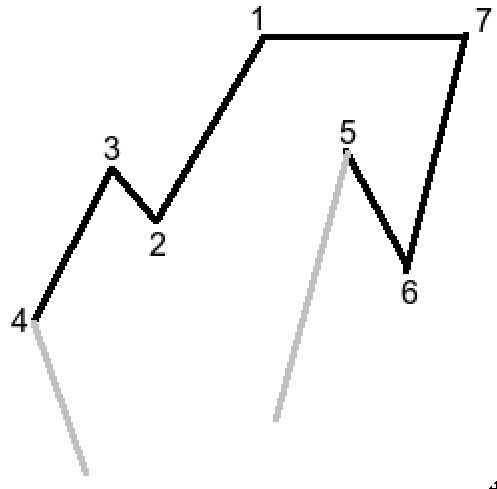
\includegraphics[width=0.5\textwidth]{figures/monotonization_example.png}
  \caption{Polygon monotonization example.}
  \label{fig:monotonization_example}
\end{figure}

}{}


\end{document}
